\documentclass[t]{beamer}

\subtitle{Section 0.4: Relations}

\usepackage{amsthm,amsmath,amsfonts,hyperref,graphicx,color,multicol,soul}
\usepackage{enumitem,tikz,tikz-cd,setspace,mathtools}

%%%%%%%%%%
%Beamer Template Customization
%%%%%%%%%%
\setbeamertemplate{navigation symbols}{}
\setbeamertemplate{theorems}[ams style]
\setbeamertemplate{blocks}[rounded]

\definecolor{Blu}{RGB}{43,62,133} % UWEC Blue
\setbeamercolor{structure}{fg=Blu} % Titles

%Unnumbered footnotes:
\newcommand{\blfootnote}[1]{%
	\begingroup
	\renewcommand\thefootnote{}\footnote{#1}%
	\addtocounter{footnote}{-1}%
	\endgroup
}

%%%%%%%%%%
%TikZ Stuff
%%%%%%%%%%
\usetikzlibrary{arrows}
\usetikzlibrary{shapes.geometric}
\tikzset{
	smaller/.style={
		draw,
		regular polygon,
		regular polygon sides=3,
		fill=white,
		node distance=2cm,
		minimum height=1in,
		line width = 2pt
	}
}
\tikzset{
	smsquare/.style={
		draw,
		regular polygon,
		regular polygon sides=4,
		fill=white,
		node distance=2cm,
		minimum height=1in,
		line width = 2pt
	}
}


%%%%%%%%%%
%Custom Commands
%%%%%%%%%%

\newcommand{\C}{\mathbb{C}}
\newcommand{\quats}{\mathbb{H}}
\newcommand{\N}{\mathbb{N}}
\newcommand{\Q}{\mathbb{Q}}
\newcommand{\R}{\mathbb{R}}
\newcommand{\Z}{\mathbb{Z}}

\newcommand{\ds}{\displaystyle}

\newcommand{\fn}{\insertframenumber}

\newcommand{\id}{\operatorname{id}}
\newcommand{\im}{\operatorname{im}}
\newcommand{\Aut}{\operatorname{Aut}}
\newcommand{\Inn}{\operatorname{Inn}}

\newcommand{\blank}[1]{\underline{\hspace*{#1}}}

\newcommand{\abar}{\overline{a}}
\newcommand{\bbar}{\overline{b}}
\newcommand{\cbar}{\overline{c}}

\newcommand{\nml}{\unlhd}

%%%%%%%%%%
%Custom Theorem Environments
%%%%%%%%%%
\theoremstyle{definition}
\newtheorem{exercise}{Exercise}
\newtheorem{question}[exercise]{Question}
\newtheorem{warmup}{Warm-Up}
\newtheorem*{defn}{Definition}
\newtheorem*{exa}{Example}
\newtheorem*{disc}{Group Discussion}
\newtheorem*{nb}{Note}
\newtheorem*{recall}{Recall}
\renewcommand{\emph}[1]{{\color{blue}\texttt{#1}}}

\definecolor{Gold}{RGB}{237, 172, 26}
%Statement block
\newenvironment{statementblock}[1]{%
	\setbeamercolor{block body}{bg=Gold!20}
	\setbeamercolor{block title}{bg=Gold}
	\begin{block}{\textbf{#1.}}}{\end{block}}
\newenvironment{thm}[1]{%
	\setbeamercolor{block body}{bg=Gold!20}
	\setbeamercolor{block title}{bg=Gold}
	\begin{block}{\textbf{Theorem #1.}}}{\end{block}}


%%%%%%%%%%
%Custom Environment Wrappers
%%%%%%%%%%
\newcommand{\enumarabic}[1]{
	\begin{enumerate}[label=\textbf{\arabic*.}]
		#1
	\end{enumerate}
}
\newcommand{\enumalph}[1]{
	\begin{enumerate}[label=(\alph*)]
		#1
	\end{enumerate}
}
\newcommand{\bulletize}[1]{
	\begin{itemize}[label=$\bullet$]
		#1
	\end{itemize}
}
\newcommand{\circtize}[1]{
	\begin{itemize}[label=$\circ$]
		#1
	\end{itemize}
}
\newcommand{\slide}[1]{
	\begin{frame}{\fn}
		#1
	\end{frame}
}
\newcommand{\slidec}[1]{
\begin{frame}[c]{\fn}
	#1
\end{frame}
}
\newcommand{\slidet}[2]{
	\begin{frame}{\fn\ - #1}
		#2
	\end{frame}
}


\newcommand{\startdoc}{
		\title{Math 425: Abstract Algebra 1}
		\author{Mckenzie West}
		\date{Last Updated: \today}
		\begin{frame}
			\maketitle
		\end{frame}
}

\newcommand{\topics}[2]{
	\begin{frame}{\insertframenumber}
		\begin{block}{\textbf{Last Section.}}
			\begin{itemize}[label=--]
				#1
			\end{itemize}
		\end{block}
		\begin{block}{\textbf{This Section.}}
			\begin{itemize}[label=--]
				#2
			\end{itemize}
		\end{block}
	\end{frame}
}

\begin{document} 
\startdoc

\topics{
	% Last Time
	\item Mappings
	\item Codomain vs Range
	\item Image and Inverse Image
	\item One-to-One, Onto, Bijection
	\item Identity Map
	\item Inverse Mappings
	\item Invertibility Theorem
}
{
	% This time
	\item Relations
	\item Equivalence Relations
	\item Equivalence Classes
}
\slide{
	\begin{defn}
		If $A$ is a set, any subset of $A\times A$ is called a \emph{relation} on $A$.
	\end{defn}
	\begin{nb}
		We often call this set $R$ and we denote the elements as $a\equiv b$.
	\end{nb}
	\begin{exa}
		\enumalph{\setlength{\itemsep}{.5in}
			\item $A=\Z$, $R=\Z\times \Z$
			
			\item $A=\R$, $a\sim b$ exactly when $a>b$
			
			\item $A=\{0,1,2\}$, $a\equiv b$ exactly when $a=b$
		}
	\end{exa}
}
\slide{
	\begin{defn}
		A relation $\equiv$ on a set $A$ is called an \emph{equivalence relation} if it satisfies all of the following conditions for all $a,b,c\in A$,
		\enumarabic{
			\item $a\equiv a$ (\emph{reflexivity}),
			\item If $a\equiv b$ then $b\equiv a$ (\emph{symmetric}),
			\item If $a\equiv b$ and $b\equiv c$, then $a\equiv c$ (\emph{transitive}).
		}
	\end{defn}
	\begin{exercise}
		For integers $m$ and $n$, say $m\equiv n$ if and only if $m-n$ is even. Show that $\equiv$ defines and equivalence relation.
	\end{exercise}
}

\slide{ 
	\begin{defn}
		Given an equivalence relation $\equiv$ on a set $A$, we define the \emph{equivalence class} of $a$ to be the set
		\[[a]=\{x\in A\ |\ x\equiv a\}.\]
	\end{defn}
	\begin{exercise}
		What are the equivalence classes from the previous exercise? ($m\equiv n$ if and only if $m-n\in2\Z$)
	\end{exercise}
}
\slide{
	\begin{exercise}
		What are the equivalence classes for each of the following relations?
		\enumalph{
			\item Equivalence given by equality.\vskip 1in\mbox{}
			\item $A=\R$, $a\equiv b$ if and only if $a^2=b^2$.\vskip 1in\mbox{}
		}
	\end{exercise}
}
\slide{
	\begin{block}{\textbf{Notation.}}
		The book uses $A_\equiv$ to be the set of unique equivalence classes of $A$ under the equivalence relation $\equiv$. 
		We may also call this set the \emph{quotient set} of $A$ by $\equiv$.
	\end{block}
	\begin{exercise}
		Let $U=\{1,2,3\}$ and $A=U\times U$.  Define the relation $\equiv$ on $A$ by $(a,b)\equiv(c,d)$ if $b=d$. 
		\enumalph{
			\item What is $A$?
			\item Show that $\equiv$ defines an equivalence relation on $A$.
			\item Determine $A_\equiv$.
		}
	\end{exercise}
}
\slide{
	\begin{defn}
		Given an equivalence $\equiv$ on a set $A$,
		the \emph{natural map} is the mapping $\phi\colon A\to A_\equiv$ given by $\phi(a)=[a]$ for all $a\in A$.
	\end{defn}
	\begin{exercise}
		Fill in the arrows for the natural map from the previous slide 
		\begin{center}
			\begin{tabular}{ccc}
				$A$& $\xrightarrow{\phi}$ & $A_\equiv$\\
				(1,1)&\hspace*{1in}&\\
				(1,2) && [(1,1)]\\
				(1,3)&&\\
				(2,1)&&\\
				(2,2) && [(2,2)]\\
				(2,3)&&\\
				(3,1)&&\\
				(2,3) && [(3,3)]\\
				(3,3)
			\end{tabular}
		\end{center}
	\end{exercise}
}
\slide{
	\begin{thm}{0.4.1}
		Let $\equiv$ be an equivalence on a set $A$ and let $a$ and $b$ denote elements of $A$. Then
		\enumarabic{
			\item $a\in [a]$ for all $a\in A$.
			\item $[a]=[b]$ if and only if $a\equiv b$.
			\item If $a\in [b]$ then $[a]=[b]$.
			\item If $[a]\neq[b]$ then $[a]\cap [b]=\emptyset$.
		}
	\end{thm}
}
\slidec{
	\begin{block}{\textbf{Brain Break.}}
		What is your preferred wallet style/type?
		\begin{center}
			
\includegraphics[height=1in]{wallet.jpg}
			\quad
			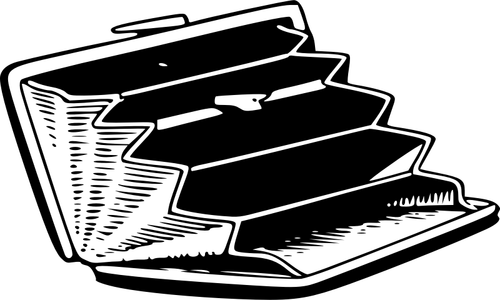
\includegraphics[height=1in]{big_wallet.png}
		\end{center}
	\end{block}
}
\slide{
	\begin{nb}
		We say that an equivalence relation \emph{partitions} a set because every element of that set will appear in \textit{exactly one} equivalence class.
		
		We call the collection of distinct equivalence classes the \emph{quotient set} of $A$ by $\equiv$.
	\end{nb}
	\begin{exercise}
		Explore this property for the equivalence relation given by $a\equiv b$ if and only if $a^2=b^2$.\vskip 3in\mbox{}
	\end{exercise}
}
\slide{
	\begin{defn}
		Two sets $X$ and $Y$ are \emph{disjoint} if $X\cap Y=\emptyset$, and a collection of sets is \emph{pairwise disjoint} if any two distinct sets in the family are disjoint.
	\end{defn}
	\begin{defn}
		If $A$ is a nonempty set and $\cal P$ is a family of subsets of $A$, we say that $\cal P$ \emph{partitions} $A$ if
		\enumalph{
			\item $\emptyset\not\in \cal P$
			\item $\cal P$ is pairwise disjoint
			\item The union of the sets in $\cal P$ is $A$
		}
	\end{defn}
}
\slide{
	\begin{exercise}
		What are all of the partitions of $\{a,b,c\}$?
	\end{exercise}
}
\slide{
	\begin{thm}{0.4.2}
		If $\equiv$ is any equivalence on a nonempty set $A$, then the collection of all equivalence classes of $A$ under $\equiv$ partitions $A$.
	\end{thm}
	\begin{exercise}
		What is the partition of $\Z$ given by $m\equiv n$ if and only if $m-n$ is even?
	\end{exercise}
}
\slide{
	\begin{exercise}
		How does this partitioning question change if we use $m\equiv n$ if and only if $m-n$ is divisible by 3?
	\end{exercise}
}
\end{document}

